\section{Von Neumannovy principy, blokové schéma Von Neumannova počítače. Rozdíl mezi Von Neumannovou, harvardskou a modifikovanou harvardskou architekturou. Procesory CISC a RISC. Rozdíl mezi obvodovým a mikroprogramovým řadičem. Řetězové zpracování instrukcí (pipelining), skokový a datový konflikt. Jak se liší a pro jaké typy úloh je určen mikroprocesor pro všeobecné použití, mikrokontrolér, signálový procesor a signálový kontrolér (DSC), SoC (System on a Chip), ASIC.}
\subsection{Von Neumnnova architektura}
\subsubsection*{Hlavní myšlenka}
Instrukce programu jsou reprezentovány binárními signály a jsou uloženy v paměti počítače spolu s daty. \\
\subsubsection*{Principy}
Principy:
\begin{itemize}
    \item Předpis pro řešení úlohy je převeden na posloupnost instrukcí
    \item Intrukce a data se nacházejí ve stejné paměti
    \item Instrukce ani data nejsou explicitně označeny
    \item Paměť je rozdělena na stejně velká paměťová místa nazývaná adresy
    \item V instrukcích není uvedena hodnota operandu, ale jeho adresa
    \item instrukce se provádějí sekvenčně
    \item Toto sekvenční provádění lze narušit instrukcemi typu skok
\end{itemize}

\begin{figure}[h!]
    \centering
    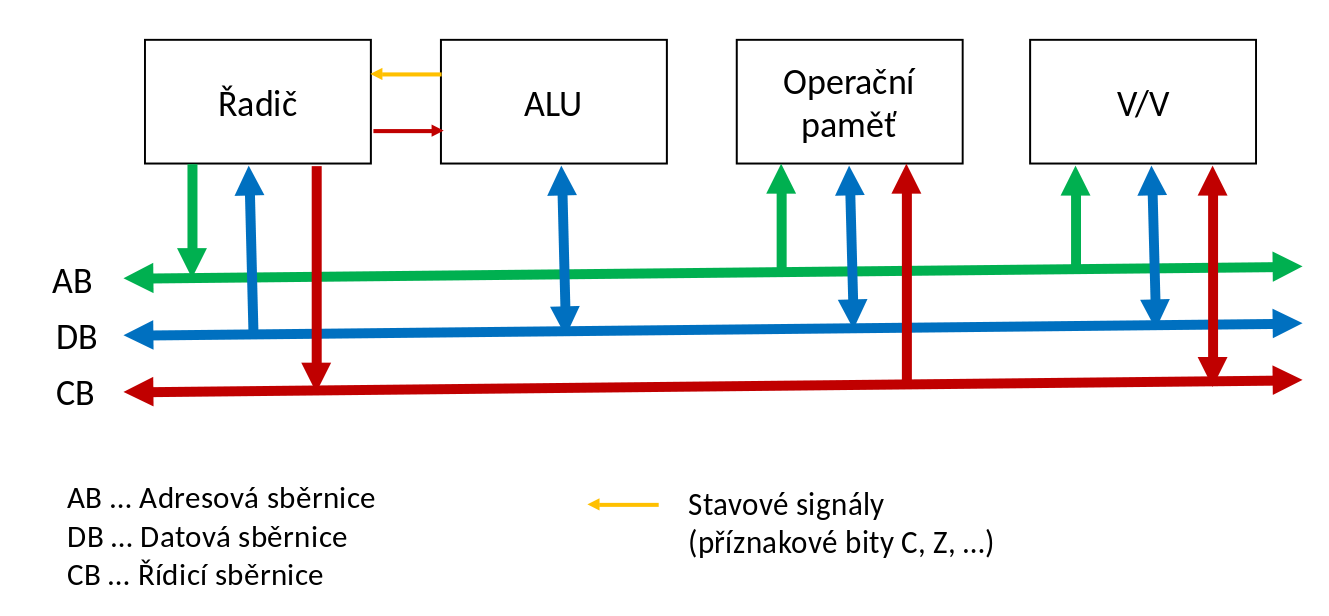
\includegraphics[width = \textwidth]{img/VonNeumann.png}
\end{figure}

\subsubsection*{Řadič}
Řídí činnost ostatních částí počítače. \\
Implementuje instrukční sadu. \\
Vstupy:\\
\begin{itemize}
    \item Signály z dekodéru instrukcí - dekóduje se část instrukce označována jako operační znak
    \item Signály generované ALU - Příznaky, přetečení, nulový výsledek, záporný výsledek
    \item Signál žádosti o obsluhu přerušení
\end{itemize}
Výstupy:\\
\begin{itemize}
    \item Čtení nebo zápis do paměti
    \item Čtení nebo zápis do periferie
    \item Signály ALU, určující kterou operaci má provést
\end{itemize}

\subsubsection*{ALU}
Aritmeticko-logická jednotka.\\
Provádí aritmetické operace(+,-,/,*), logické operace(AND,OR,NOT) a operace porovnání(>,<,=)\\
Řadič a ALU tvoří CPU. Integrací řadiče, ALU a registrů na jeden čip vzniká mikroprocesor.

\subsubsection*{Operační paměť}
Místo uložení dat a instrukcí.\\
Společná paměť pro instrukce a data. Jsou uloženy v jednom paměťovém prostoru.\\
U mikrokontrolerů jsou v instrukce v paměti FLASH a proměnné v paměti RAM, ale obě jsou připojeny ke stejným sběrnicím(AB,CB,DB)

\subsubsection*{V/V}
Slouží pro komunikaci s okolím.\\
Člověkem - klávesnice, myš, obrazovka. \\
Strojem, přístrojem či technologickým procesem - I/O, A/D, D/A převodníky a k nim akční členy - snímače. \\
S ostatními počítači a zařízeními pomocí sítě - Ethernet, WiFi moduly. \\
Umožňují ukládání dat na disky(SSD, HDD). \\

\subsubsection*{Registry}
Typy registrů:
\begin{itemize}
    \item Pracovní registr
          \begin{itemize}
              \item Ukládají operandy z ALU a výsledky z ALU
              \item Rychlejší než operační paměť
              \item Původně jeden registr nazývaný akumulátor
          \end{itemize}
    \item Stavový registr
          \begin{itemize}
              \item Skupina klopných obvodů ovládaných ALU
              \item Uchovávají stav ALU mezi instrukcemi
              \item Příznaky přetečení/výpůjčky, nulového či záporného výsledku
              \item Předcházející instrukce příznaky nastaví, následující využije
          \end{itemize}
    \item Programový čítač
          \begin{itemize}
              \item Zajišťuje sekvenční provádění instrukcí a provádění skoků
              \item V průběhu zpracování instrukce se nastaví tak aby obsahoval adresu následující instrukce
          \end{itemize}
\end{itemize}
Řídící a stavový registr bývají spojeny do jednoho řídícího stavového registru.\\

\subsubsection{Cyklus počítače}
Celý cyklus práce počítače se dělí na tyto opakující se části.
\begin{enumerate}
    \item Intruction fetch - načtení instrukce z paměti
    \item Intruction decode - dekódování instrukce
    \item Operand fetch - načtení operandu z registrů
    \item Intruction expectation
    \item Write-back (Result store) - uložení výsledku
    \item Test, není-li požadavek na přerušení
\end{enumerate}
Nemusí se nutně vykonávat všechny tyto fáze.\\
Povinné fáze jsou pouze 1,2,4.

\subsection{Rozdíly mezi VonNeumannovou, harvardskou a modifikovanou harvardskou architekturou}
\subsubsection*{Von Neumannova architektura}
Společná paměť pro instrukce a data. \\
Existuje jedna datová a jedna adresová sběrnice. \\
Pomalejší oproti HA a MHA kvůli nutnosti číst instrukce nebo operand. \\
Výhoda spouštění programů z disků, jednoduchá změna počítače. \\
Dobře využitelná paměť. \\
Poloviční počet sběrnic oproti HA. Jednodušší konstrukce. \\
\begin{figure}[h!]
    \centering
    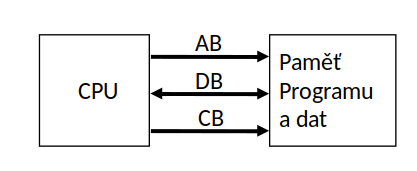
\includegraphics[]{img/VNporovnani.png}
\end{figure}

\subsubsection{Harvardská architektura}
Oddělena paměť dat a programu. To umožňuje číst obě zaráz a urychluje práci.\\
Může být různě adresována datová paměť a programová paměť.\\
Bezpečnější, nelze si poškodit program přepsáním jeho paměti.\\
Dvojnásobek sběrnic oproti VN, technilogicky velký problém. \\
Nevyužitou část paměti nejde použít pro program a naopak. Z toho plyne, že je nižší efektivita využití paměti. \\
Využívá se u signálových procesorů, jinak moc ne.\\
\begin{figure}[h!]
    \centering
    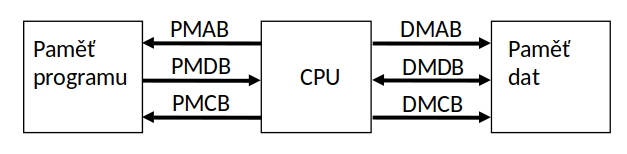
\includegraphics[width = \textwidth]{img/HAporovnani.png}
\end{figure}

\subsubsection*{Modifikovaná harvardská architektura}
Stejně jako HA 2 paměti. S rozdílem toho, že jedna je čistě pro data a druhá pro data a program.\\
Umožňuje číst 2 operandy zároveň díky rozmístění paměti. Toto umožňuje operaci Multiply and accumulate. \\
Využívá se u signálových procesorů a kontrolerů. \\

\begin{figure}[h!]
    \centering
    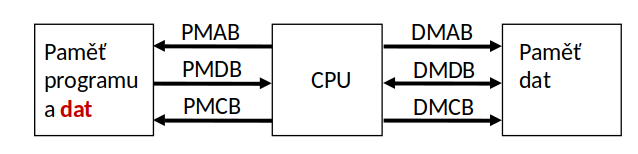
\includegraphics[width = \textwidth]{img/MHAporovnani.png}
\end{figure}

\subsection{Obvodový a mikroprogramový řadič}
\subsubsection*{Obvodový řadič}
Synchronní konečný stavový automat.\\
Logické členy a klopné obvody. \\
Umožňuje malou sadu jednoduchých instrukcí. \\
Výhodou je jednoduchost a malý počet součástek. \\
Nevýhodou je nutnost složité operace rozdělovat na více instrukcí. \\

\subsubsection*{Mikroprogramový řadič}
KSA, jehož paměť je tvořena pamětí mikroprogramu. \\
Implementuje složité instrukce za cenu složitosti řadiče. \\
Složité instrukce není možné přímo provést, proto jsou rozděleny na mikroinstrukce. \\
Posloupnost mikroinstrukcí, jimiž se vykoná instrukce se nazývá mikroprogram. \\
Mikroprogramy pro jednotlivé instrukce jsou uloženy v paměti mikroprogramu. \\
Toto zvyšuje složitost řadiče a počet cyklů potřebných na provedení instrukce. \\
Nutno operovat v nižších frekvencích kvůli problému s odvodem tepla. \\

\subsection{Procesory CISC a RISC}
\subsubsection*{CISC}
Complex instruction set computer. \\
Složité instrukční sady, přizůsobené tak aby realizovaly příkazy programovacího jazyka. \\
Používá mikroprogramový řadič. \\
Stovky instrukcí. \\
Přesun složitosti z SW do HW. \\

\subsubsection*{RISC}
Reduced instruction set computer. \\
Malý počet jednoduchých instrukcí. \\
Vyšší nároky na překladače z programovacích jazyků. \\
Instrukce mají konstatní délku a jednotný formát, který vymezuje počet bitů v instrukci. \\
Obvodový řadič. \\
Velký počet registrů(16+), to snižuje nutnost častého přístupu do operační paměti. \\
Jediné instrukce, které mají povoleno interagovat s pamětí jsou \texttt{load} a \texttt{store}, load z paměti do registru, store naopak. Ostatní instrukce pracují pouze s registry.\\
V každém hodinovém taktu dokončena jedna instrukce. \\
Používá pipelining. \\

\subsubsection*{Post-RISC}
Kombinace CISC a RISC. \\
Rozšiřuje RISC o instrukce, které lze provádět rychle. \\
Hluboká pipeline až 10 kroků. \\
Více ALU pracujících paralelně. \\

\subsection{Řetězové zpracování instrukcí - pipelining}
Efektivnější využití času. \\
Každá fáze využívá jinou část CPU -> návrh procesoru pro paralelní práci na jeho částech. \\

\begin{figure}[h!]
    \centering
    \begin{minipage}[b]{0.4\textwidth}
        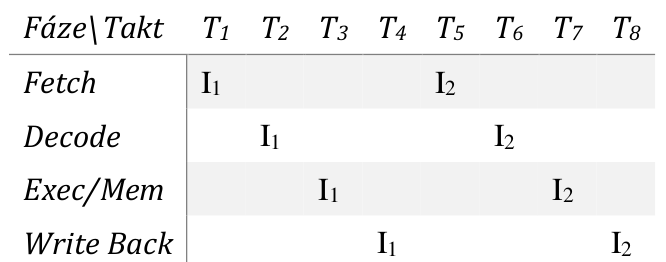
\includegraphics[width=\textwidth]{img/sekv.png}
    \end{minipage}
    \hfill
    \begin{minipage}[b]{0.4\textwidth}
        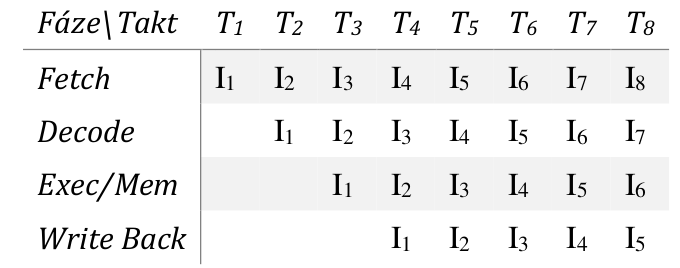
\includegraphics[width=\textwidth]{img/pipeline.png}
    \end{minipage}
\end{figure}

Doba exekuce instrukcí, kde k je počet fází:
\begin{center}
    Pipelining: $N = k + (n-1)$\\
    Sekvenční: $M = n \cdot k$ \\
    Koeficient zrychlení: $S_k = \frac{M}{N} = \frac{n \cdot k}{n + n-1}$
\end{center}

\subsection{Skokový konflikt}
Při instrukci větvení nebo přerušení. Ve chvíli kdy se začne provádět skok jsou v řetězci rozpracované instrukce. Řetězec tudíž musí být vyprázdněn a znovu naplněn, což vede ke snížení efektivity.\\
Řešení:
\begin{itemize}
    \item Predikce skoků
          \begin{itemize}
              \item Statická - nebere v úvahu historii provádění příslušné operace skoku. Například při provádění cyklu se skok provede vždy, instrukce obsahuje bit, který nastaví překladač (překladač odhaduje pravděpodobnost skoku)
              \item Dynamická - snaží se předpovědět skoky na základě chování programu v minulosti. Například provedl-li se skok při minulé exekuci dané instrukce počítá se, že se provede znovu. Procesor musí být vybaven spekulativní jednotkou
          \end{itemize}
    \item Použití dvou řetězců - 2 řetězce, jeden pro sekvenční provádění a druhý pro skoky.
\end{itemize}

\subsection{Datový konflikt}
Pokud instrukce pracuje s operandem z předchozí instrukce, která se však ještě nedokončila. \\

\begin{figure}[h!]
    \centering
    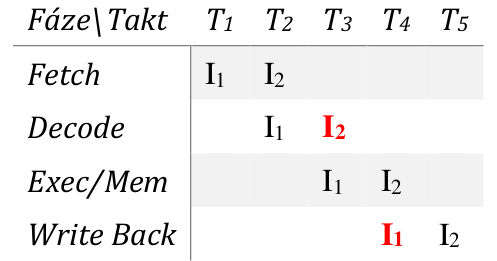
\includegraphics[scale = 0.4]{img/datKonf.png}
\end{figure}

Řešení:
\begin{itemize}
    \item Překladač řadí instrukce tak aby ke konfliktu nedošlo.
    \item Procesor detekuje konflikt a pozastaví konání $I_2$. Snižuje účinost řetězení.
    \item Procesor detekuje konflikt a změní pořadí instrukcí. Náročné na konstrukci procesoru.
\end{itemize}

\subsection{Superpipelined procesor}
Procesor rozdělený na subprocesory, které zpracovávají instrukce jako řetězec. \\
Subprocesory je možné dělit na subbloky, které tvoří řetězce subprocesorů. \\

\subsection{Mikroprocesor, mikrokontrolér, signálový procesor, signálový kontroler,SOC, ASIC}
\subsubsection{Mikroprocesor pro všeobecné využití}
Na jednom čipu ALU, řadič, registry, případně cache a MMU.\\
Velký výpočetní výkon a paměťový prostor.\\
Stolní PC, notebooky, servery.\\
Modifikace pro telefony a tablety, optimalizovány na nízkou spotřebu, nižší výkon a paměť. \\

\subsubsection*{Mikrokontrolér}
Základní stavební kámen vesvných zařízeních. \\
Na jednom čipu procesor (řadič, ALU, registry, případně cache a MMU), paměti RAM a FLASH, řadič přerušení a periferie.\\
Menší výkon a paměť.\\
Určen pro embedded aplikace, spotřební elektronika, průmysl, automobily, řídící aplikace. \\

\subsubsection*{Signálový procesor - DSP}
Vznikly pro číslicové zpracování signálů v reálném čase a spektrální analýzu. \\
Vyžadují rychlé provádění specifických výpočetních operací, ale nepotřebují moc paměti. Například multiply and accumulate, v podstatě konvoluce, součin dvou parametrů a přičtení k proměnné.\\
Méně periferií než mikrokontroléry. \\
Dělí se na 2 typy:
\begin{itemize}
    \item S pevnou řádovou čárkou - jednodušší, levnější, algoritmy se hůře implementují
    \item S plovoucí řádovou čárkou, dražší, ale jednodušší implementace
\end{itemize}

\subsubsection*{Signálový kontroler - DSC}
Kombinace DSP a mikrokontroleru.\\
Má více periferií oproti DSP. \\
Využití pro výkonovou elektroniku. Měniče, vektorové řízení motorů.\\

\subsubsection*{System on a chip - SoC}
Integrovaný obvod, který zahrnuje všechny části počítače na jeden čip. \\
Digitální, analogové, rádiové, smíšené obvody na jednom čipu. \\

\subsubsection*{ASIC}
Integrovaný obvod navržený pro jednu aplikaci.\\
Většinou digitální, hromadná výroba.\\

\section{Rozdíl mezi izolovanými a paměťově mapovanými periferiemi. Způsoby obsluhy V/V: aktivní čekání, přerušení, DMA.
  Přerušení: řadič přerušení, činnost procesoru při zahájení obsluhy přerušení a návratu z přerušení, tabulka vektorů přerušení. Asynchronní a synchronní přerušení. Maskovatelné, nemaskovatelné a pseudomaskovatelné přerušení. Vnořené přerušení. RESET, činnost procesoru po RESETu.}
\subsection{Izolované a paměťově mapované periferie}
\subsubsection{Izolované}
Periferie využívají samostatný adresový prostor oddělený od adresového prostoru operační paměti.\\
Pro přístup k izolovaným periferiím se používají speciální instrukce.\\
Intel procesory mají společnou AB a DB pro periferie i operační paměť. Intrukce IN a OUT.

\subsubsection*{Paměťově mapované}
Periferie se nacházejí ve stejném paměťovém prostoru jako operační paměť. \\
Pro přístup k periferiím se používají stejné instrukce jako pro přístup k operandům v operační paměti.\\
\subsection{Způsob obsluhy V/V}
\subsubsection*{Řídící registry periferií}
Různé periferie se značně liší, ale práce s nimi je do jisté míry podobná.\\
Z hlediska programátora jsou důležité registry periferií, které se podle funkce dají rozdělit:
\begin{itemize}
    \item Konfigurační (řídící) registry - slouží pro nastavení režimu fungování periferie.
    \item Stavové (příznakové) registry - obsahují příznakové bity (flagy), které signalizují stav periferie (např. stavový registr A/D převodníku obsahuje bit signalizující dokončení převodu)
    \item Datové registry - slouží pro vyčítání nebo ukládání dat, které periferie zpracovává
\end{itemize}

\subsubsection*{Obsluha pomocí aktivního čekání - busy waiting, pooling}
Procesor odstartuje V/V operaci zápisem do řídícího nebo datového registru a pak ve smyčce testuje, zda-li byla operace dokončena nebo došlo k chybě - to značí příslušný bit (flag).\\
Velká nevýhoda je, že během čekání ve smyčce procesor nemůže provádět jinou užitečnou činnost => plýtvání času.\\
V embedded systémech hrozí, že dojde k promeškání důležité události (např. nárust tlaku v nádobě => havárie).\\
Jediná výhoda je jednoduchá implementace, využívá se při testování u vývoje periferií.\\

\subsubsection*{Obsluha pomocí přerušení}
Procesor odstartuje V/V operaci zápisem do řídícího nebo datového registru. \\
Nečeká na dokončení operace, ale provádí jinou užitečnou činnost.\\
Po dokončení operace nebo při chybě periferie generuje požadavek na přerušení.\\
Procesor rozpozná požadavek na přerušení a dočasně přeruší provádění aktuálního kódu a vykoná kód obslužné rutiny přerušení pro danou periferii. \\
Po vykonání obslužné rutiny se procesor opět vrátí k vykonávání kódu, který prováděl před přechodem do přerušovací rutiny.\\

\subsubsection*{Obsluha pomocí DMA}
Některé periferie (např. řadiče disků) obsahují vyrovnávací paměti.\\
Při provádění V/V operací je třeba přenášet větší množství bytů mezi operační pamětí a vyrovnávací pamětí periferie. \\
Je výhodné, aby přenos dat probíhal bez účasti procesoru a procesor mohl provádět jinou užitečnou činnost. Aby toto bylo možné musí v počítači být řadič sběrnic - DMA. Během přenosu dat CPU uvolní sběrnice a ty převezme řadič DMA. DMA generuje adresy a řídící signály jako MEMR a MEMW.
Před zahájením DMA přenosu musí procesor na DMA nakonfigurovat:
\begin{itemize}
    \item Počáteční adresu v operační paměti.
    \item Počáteční adresu v paměti periferie.
    \item Směr přenosu.
    \item Počet přenášených bytů.
\end{itemize}

\subsection{Přerušení}
\subsubsection*{Použití přerušení}
Používá se pro obsluhu neodkladných událostí. \\
Při požadavku na přerušení procesor přeruší aktuálně prováděný kód a provede kód obsluhující událost a vrátí se zpět.\\
Kód obsluhy se nazývá obslužná rutina přerušení.\\
Používá se pro obsluhu periferií, nebo k ošetření výjimečných situací jako chyby a havarijní stavy (např. dělení nulou, chyba ochrany paměti, pokles napájecího napětí atd.).\\
Přerušení lze také vyvolat softwarově pomocí příslušné instrukce. Používá se pro přístup ke službám jádra operačního systému. Na některých procesorech je to jediný způsob, jak lze přejít z uživatelského módu na mód supervisor (v němž běží jádro operačního systému)

\subsubsection*{Řadič přerušení}
Počítač obvykle používá více V/V periferií, které mohou generovat požadavky na přerušení.\\
Jednotlivé zdroje přerušení jsou připojeny na vstupy bloku počítače nazývaného řadič přerušení.\\
Aby procesor mohl určit zdroj přerušení, je ke každému zdroji přiřazeno celé kladné číslo. Periferie nastaví aktivní úroveň signálu na vstup řadiče a ten zašle číslo přerušení. Periferie mají z hlediska obsluhy různou prioritu, podle toho se řadič rozhoduje, co oznámí procesoru jako první, když je současně generováno víc požadavků.\\
Priorita buď softwarově nebo hardwarově, softwarovou můžeme měnit zápisem do řadiče.\\
Dnešní počítače vybavené sběrnicí PCI Express nepoužívají dedikované vodiče pro komunikaci mezi řadičem a procesorem, periferie posílají požadavek na obsluhu jako zprávu po sběrnici PCIe. Zpráva je posílána na speciální adresu v paměťovém prostoru. Tento způsob přerušení se nazývá MSI ( Message Signaled Interrupts).

\subsubsection*{Činnost procesoru při obsluze přerušení}
Při příchodu požadavku na asynchronní nebo softwarové přerušení procesor dokončí prováděnou instrukci. \\
Na konci instrukčního cyklu procesor testuje, jestli není požadavek na obsluhu přerušení, pokud je, tak procesor zahájí obsluhu:
\begin{enumerate}
    \item Uloží do zásobníku návratovou adresu
    \item Uloží do zásobníku obsah stavového registru
    \item Některé procesory ukládají do zásobníku obsah pracovních registrů
    \item V příznakovém registru nastaví bit I, čímž zakáže přerušení. Během provádění obslužné rutiny jsou maskovatelná přerušení zakázána, pokud je programátor v přerušovací rutině explicitně nepovolí
    \item Procesor na základě čísla přerušení stanoví adresu vektoru přerušení. Na adrese vektoru přerušení se musí nacházet adresa první instrukce obslužné rutiny
    \item Procesor vyzvedne adresu první instrukce z vektoru přerušení a vloží ji do programového čítače - tím se začne provádět obslužná rutina
\end{enumerate}
Poslední instrukce obslužné rutiny přerušení musí být instrukce návratu z přerušení (RTI), která zajistí, že procesor:
\begin{itemize}
    \item Pokud procesor uložil obsah pracovních registrů, obnoví jejich obsah
    \item Obnoví ze zásobníku obsah stavového registru - tím se povolí maskovatelná přerušení (nastavení bitu I)
    \item Vyzvedne ze zásobníku návratovou adresu a vloží ji do programového čítače, v případě asynchronního přerušení procesor pokračuje následující instrukcí, u výjimek (např. dělení nulou) se restartuje instrukce, která výjimku způsobila
\end{itemize}
Pokud má procesor větší množství pracovních registrů, ukládání pracovních by trvalo nepřijatelně dlouho, přitom by programátor nebo překladač obsah některých registrů v přerušovací rutině nemodifikoval. Proto procesory s větším množství registrů tyto registry automaticky neukládají a je odpovědnost programátora nebo překladače uložit ty registry, které se budou modifikovat.\\
Existují procesory, které mají pracovní registry zdvojené a jen se přepíná mezi hlavními a stínovými(pro rutinu) registry. Přepínání je rychlé, ale velmi náročné na konstrukci. Toto řešení je dnes spíše výjimkou. \\

\subsubsection*{Vektor přerušení}
Adresa kde se nachází první instrukce obslužné rutiny.\\
Každý zdroj přerušení má svůj vektor přerušení.\\

\subsubsection*{Tabulka vektorů přerušení}
Oblast paměti kde jsou za sebou umístěny vektory přerušení.\\
Číslo vektoru je indexem tabulky vektorů.\\
Řadič předá procesoru číslo vektoru přerušení, procesor vynásobí číslo vektoru přerušení velikostí vektoru přerušení a výsledek přičte k adrese začátku tabulky vektorů přerušení.\\
Počáteční adresa tabulky bývá u jednoduchých procesorů daná výrobcem napevno, složitější na to mají speciální registr, kde se napíše námi zvolená adresa.

\subsubsection*{Asynchronní a synchronní přerušení}
\begin{itemize}
    \item Asynchronní
          \begin{itemize}
              \item nejsou synchronizovány s prováděním instrukcí v CPU
              \item jsou vyvolány asynchronními událostmi
              \item typické zdroje jsou V/V periferie - dokončení AD převodu, doběhnutí časovače, příjem ethernet rámce, zmáčknutí klávesy, detekce poklesu napětí
          \end{itemize}
    \item Synchronní
          \begin{itemize}
              \item Generována v důsledku provádění určitých instrukcí v přesně definované fázi zpracování dané instrukce.
              \item Přerušní generují instrukce softwarového přerušení a výjimky
              \item Výjimky jsou generovány kontrolními obvody počítače, když dojde k chybě v provádění instrukce. Typické výjimky jsou dělení nulou, pokus o exekuci neznámé či ilegální instrukce, noprávněný pokud o přístup k paměti
          \end{itemize}
\end{itemize}

\subsubsection*{Maskovatelná přerušení}
Přerušení lze povolit nebo zakázat obvykle nastavením (vynulováním) bitu I v příznakovém registru.\\
Např. Program provádí úsek kódu kde pracuje s proměnnými, které používá přerušovací rutina, před začátkem práce s těmito proměnnýma zakáže přerušení a provede manipulaci a pak opět povolí přerušení.\\

\subsubsection*{Nemaskovatelná přerušení}
Kritické události jako porušení paměti nebo výpadek napájení je však třeba obsloužit vždy. \\
Tyto přerušení musí být povolena vždy a nesmí být možnost je zakázat.\\
Například porušení paměti či výpadek napájení. \\

\subsubsection*{Pseudomaskovatelná přerušení}
U nemaskovatelných vznikal problém při zahájení činnosti procesoru po RESETu. Obsluha přerušení vyžaduje minimálně nastavení ukazatele zásobníku na adresu začátku zásobníku  v paměti RAM. Vyvolání přerušení v okamžiku, kdy není nastaven ukazatel může způsobit zhroucení celého systému. Proto je potřeba po dobu základní inicializace zabránit obsluze jakýchkoliv přerušení, tedy i nemaskovatelných. \\
Toto přerušení je po resetu zakázáno, ale po inicializaci systému se přerušení povolí a do dalšího resetu jej nejde zakázat a chová se jako nemaskovatelné. \\

\subsubsection*{Vnořená přerušení}
Může nastat situace, kdy procesor provádí obslužnou rutinu přerušení a během ní dojde požadavek na další přerušení. \\
Pokud mají stejnou prioritu, tak se první provede jedna a pak až druhá obsluha.\\
V praxi to tak ale většinou není, většinou jedno přerušení má větší prioritu. Takže uprostřed prvního přerušení se provede druhé přerušení (vnořené) a po vykonání se vrátí k prvnímu a to se dokončí.\\
\subsection{RESET a činnost procesoru po RESETu}
RESET procesoru způsobí nastavení procesoru do definovaného výchozího stavu.\\
Z hlediska uživatele to znamená, že se vynulují pracovní registry a řídící registry se nastaví na výrobcem definované hodnoty.\\
Po uvolnění signálu RESET procesor vyzvedne z definované adresy reset vektor adresu první instrukce a vloží ji do programového čítače.\\
Adresa reset vektoru je definována výrobcem a musí být v pevné paměti.\\
Stejně tak musí být první instrukce uložena v pevné paměti. Dnes uloženy ve FLASH paměti kde je UEFI, které provádí incializaci V/V periferií a zavedení OS.\\
U jednoduchých kontrolerů bývá reset poslední vektor v tabulce přerušení.\\

\section{Princip a vlastnosti pamětí ROM, EEPROM, FLASH. Rozdíl mezi paměťmi NOR FLASH a NAND FLASH. Princip pamětí MRAM a FeRAM.}

\section{Princip a vlastnosti statických pamětí RAM (SRAM) a dynamických pamětí RAM (DRAM), synchronní paměti DRAM (SDRAM).
  Připojování paralelních pamětí SRAM, FLASH ke sběrnicím mikroprocesoru. Adresový dekodér.
  Hierarchie paměti, paměti cache, specializované paměti cache.}

\section{Pojem logická a fyzická adresa, ochrana paměti, memory management unit (MMU). Stránkování (princip, transformace logické adresy na fyzickou, stránkovací tabulka). Virtuální adresový prostor. Zrychlení překladu adres pomocí Translation Look-aside Buffer (TLB).}